\documentclass{article}

% set font encoding for PDFLaTeX or XeLaTeX
\usepackage{ifxetex}
\ifxetex
  \usepackage{fontspec}
\else
  \usepackage[T1]{fontenc}
  \usepackage[utf8]{inputenc}
  \usepackage{lmodern}
  \usepackage{graphicx}
\fi

% used in maketitle
\title{Evaluacion 2}
\author{Cabello Lopez Marco Antonio\\
Departamento de Fisica \\
Universidad de Sonora}
\date{Hermosilo, Sonora a Viernes 1 de Diciembre del 2017}


% Enable SageTeX to run SageMath code right inside this LaTeX file.
% documentation: http://mirrors.ctan.org/macros/latex/contrib/sagetex/sagetexpackage.pdf
% \usepackage{sagetex}

\begin{document}
\maketitle
\clearpage

\section{Problema 1: Taylor}
\begin{verbatim}
program taylor

    implicit none                  
real (kind=8) :: x, exp_true, y
    real (kind=8), external :: exptaylor
    integer :: n

    n = 20               ! number of terms to use
    x = 1.0
    exp_true = exp(x)
    y = exptaylor(x,n)   ! uses function below
    print *, "x = ",x
    print *, "exp_true  = ",exp_true
    print *, "exptaylor = ",y
    print *, "error     = ",y - exp_true

end program taylor

!==========================
function exptaylor(x,n)
!==========================
    implicit none

    ! function arguments:
    real (kind=8), intent(in) :: x
    integer, intent(in) :: n
    real (kind=8) :: exptaylor

    ! local variables:
    real (kind=8) :: term, partial_sum
    integer :: j

    term = 1.
    partial_sum = term

    do j=1,n
        ! j'th term is  x**j / j!  which is the previous term times x/j:
        term = term*x/j   
        ! add this term to the partial sum:
        partial_sum = partial_sum + term   
        end do
     exptaylor = partial_sum  ! this is the value returned
end function exptaylor
\end{verbatim}
Resultados:  x =    1.0000000000000000    \\
exptrue  =    2.7182818284590451 \\
exptaylor =    2.7182818284590455    \\
error     =    4.4408920985006262E-016 \\
Es la diferencia entre el valor "verdadero" de la funcion y el valor usando la serie de taylor en determinado punto.
\clearpage

\section{Problema 2: Exponencial}
\begin{verbatim}
SUBROUTINE EXPTAYLOR (n, j, fi, fj, expt)
	integer, intent (IN)      :: n
	double precision, intent (IN) :: fi
	integer :: j
	double precision, dimension (100), intent(OUT) :: expt
	double precision :: fj, termino, sumaparcial
	
	
	
	termino = 1
	sumaparcial = termino
	DO j = 1, n
	 fj = dble(j)
	 termino = termino * fi / fj
	 sumaparcial = sumaparcial + termino
	 expt(j) = sumaparcial
	END DO

	 
END SUBROUTINE EXPTAYLOR
	 

PROGRAM EXPONENCIAL
	double precision, dimension (15) :: f
	integer :: i, j, n
	double precision, dimension (100)   :: x
	double precision, dimension (100) :: expt
	double precision, dimension (100) :: funcion
	double precision :: fi, fj, termino, sumaparcial

     OPEN (1, FILE = 'exp.dat', STATUS = 'unknown')
	
	DO n=1, 15, 2
	DO i=0, 100, 1
	  fi = dble(i)
	  fi = fi / 10.0d0
	CALL EXPTAYLOR(n, j, fi, fj, expt)
	funcion(n) = expt(n)
	WRITE(1,*) fi, funcion(n)

	END DO
	WRITE (1,*) ' '
	END DO
     CLOSE (1)

END PROGRAM EXPONENCIAL

\end{verbatim}

\begin{figure}
  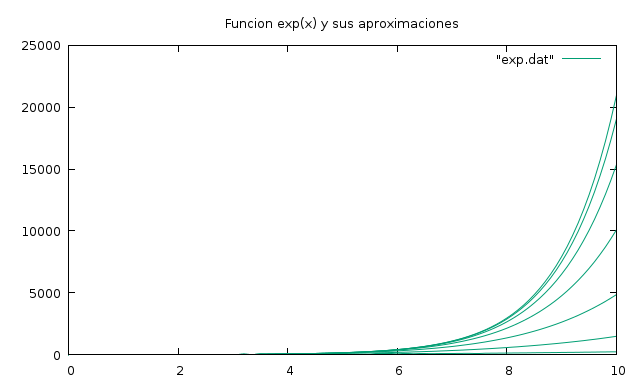
\includegraphics[width=\linewidth]{aproximacioneexp.png}
  \caption{Aproximaciones exp(x)}
\end{figure}


\clearpage




\section{Problema 3: Seno}
\begin{verbatim}
SUBROUTINE FUNCIONSENO (n, j, fi, fj, seno, signo, potencia, factorial)
	integer, intent (IN)      :: n
	double precision, intent (IN) :: fi
	integer :: j
	double precision, dimension (10000), intent(OUT) :: seno
	double precision :: fj, termino, sumaparcial, signo, potencia, factorial

	
	signo = 1.0d0
	termino = fi
	sumaparcial = termino
	potencia = fi
	factorial = 1
	DO j = 1, n
	 fj = dble(j)
	 potencia = fi**(j + 2)
	 factorial = factorial * (j + 1) * (j + 2)
	 signo = signo * (-1.0d0)
	 termino = potencia / factorial
	 termino = termino * signo
	 sumaparcial = sumaparcial + termino
	 seno(j) = sumaparcial
	 
	END DO

	 
END SUBROUTINE FUNCIONSENO
	 

PROGRAM APROXIMACIONESSENO
	double precision, dimension (10000) :: f
	integer :: i, j, n
	double precision, dimension (10000)   :: x
	double precision, dimension (10000) :: seno
	double precision, dimension (10000) :: funcion
	double precision :: fi, fj, termino, sumaparcial, signo, potencia, factorial
	

     OPEN (1, FILE = 'funciones.dat', STATUS = 'unknown')
	fi = -3.1d0
	DO i=1, 60
	WRITE (1,*) fi, fi
	fi = fi + 0.1d0
	
	END DO
	WRITE (1,*) ' '
	DO n=1, 15, 2
	  fi = -3.1d0
	DO i=1, 60
	fi = fi + 0.1d0
	CALL FUNCIONSENO (n, j, fi, fj, seno, signo, potencia, factorial)
	funcion(n) = seno(n)
	WRITE (1,*) fi, funcion(n)

	END DO
	WRITE (1,*) ' '
	END DO
     CLOSE (1)

END PROGRAM APROXIMACIONESSENO
\end{verbatim}

\begin{figure}[h!]
  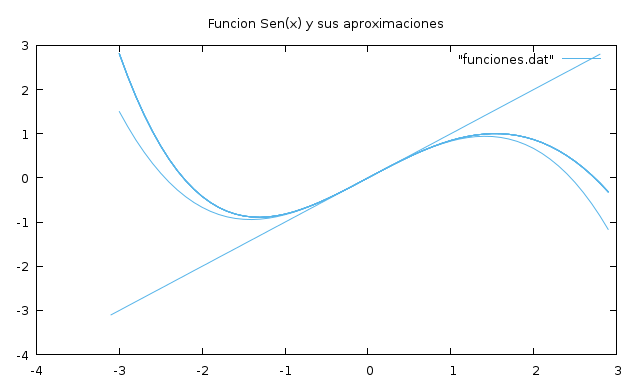
\includegraphics[width=\linewidth]{aproximacionessenos.png}
  \caption{Aproximaciones Sen(X)}
  \label{fi}
\end{figure}



\end{document}